\documentclass{article}
\usepackage{iclr2027_conference,times}
\usepackage[hidelinks]{hyperref}
\usepackage{url}
\usepackage{amsmath,amssymb,amsfonts}
\usepackage{booktabs}
\usepackage{graphicx}
\usepackage{xcolor}
\usepackage{multirow}
\usepackage{enumitem}
\usepackage{amsthm}
\usepackage{microtype}
\usepackage{mathtools}
\usepackage{tikz}
\usetikzlibrary{arrows.meta,positioning}
\definecolor{greenaccent}{HTML}{17865C}
\definecolor{redaccent}{HTML}{B4433D}
\definecolor{blueaccent}{HTML}{3568A8}
\definecolor{softgray}{HTML}{F3F4F6}
\newtheorem{proposition}{Proposition}
\newtheorem{theorem}{Theorem}
\newtheorem{corollary}{Corollary}
\newcommand{\R}{\mathbb{R}}
\newcommand{\JW}{\textsc{Joint Witness}}
\newcommand{\green}{\textsc{Green}}
\newcommand{\pat}{\mathrm{PAT}}
\newcommand{\tar}{\mathrm{TAR}}
\newcommand{\rms}{\operatorname{RMS}}

\title{When Restoration Lies:\\
Certifying Local Mechanistic Transport in Transformers}
\author{Anonymous}
%\iclrfinalcopy
\begin{document}
\maketitle

\begin{abstract}
Activation patching is often treated as mechanistic evidence: if a clean activation restores a model's answer, the patched computation is presumed to match the natural one. The output alone cannot identify that claim. We show why three plausible repairs fail under targeted stress tests. Activation overlap changes with the reference distribution; multidirectional response agreement can coexist with failure of a selected structural readout; and a response-only estimator with median joint error $3.35\times10^{-7}$ still produced deterministic intervals that crossed zero on all 80 records. These failures motivate \green{}, a certificate for a narrower, explicit object: \emph{local matched-bypass transport equivalence}. \green{} represents four patched/target and joint/bypass branches in one shared causal-cone program, propagates outward interval jets through the frozen Transformer tail, and preserves exact relational cancellation. A signed-secant construction and independent 384/512-bit replay yield five total statuses that separate certified agreement, certified disagreement, proof uncertainty, invalid execution, and exhausted compute. The guarantee concerns a declared local path functional, not a unique true mechanism. We test scientific usefulness prospectively: on IOI and Greater-Than, \green{} commits statuses before a sealed full-response endpoint is opened and is compared at matched coverage with patching, attribution, integrated-gradient, Hessian, signal-to-noise, divergence, and generic-verification baselines. The method, falsification evidence, and analysis are complete at this snapshot; the untouched successor confirmation remains sealed.
\end{abstract}

\section{Introduction}
\label{sec:intro}

Activation patching changes an internal state and measures whether the model's output changes or recovers \citep{vig2020investigating,zhang2024best}. Its causal intervention is real, but the common interpretation is too strong: recovering the answer does not identify which computation produced it. A patch can recruit a dormant route \citep{makelov2024illusion}, create a divergent representation \citep{grant2026addressing}, or mix a mediator contribution with bypass interactions \citep{vaidyanathan2026mediators}. We call the resulting failure mode a \emph{restoration lie}: the behavioral conclusion is correct, while the intended local mechanistic conclusion is not established.

\begin{figure}[b]
\centering
\resizebox{\textwidth}{!}{%
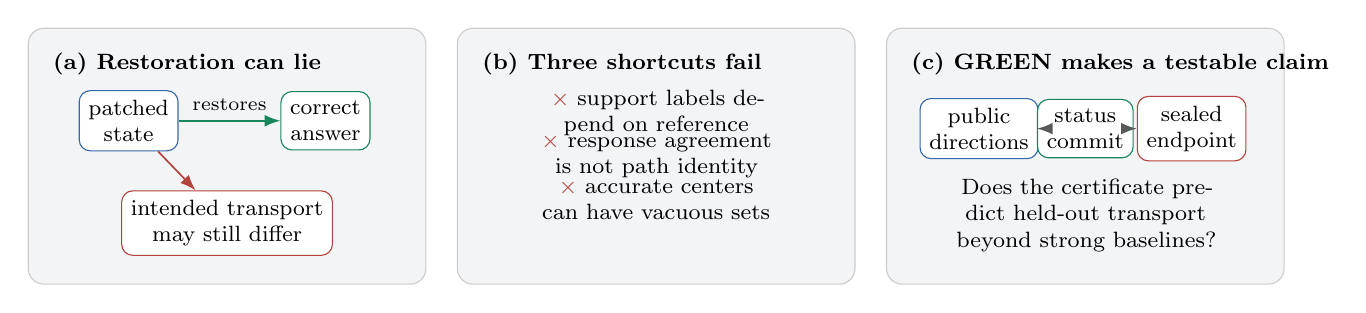
\begin{tikzpicture}[
    font=\small,
    panel/.style={draw=black!20, rounded corners=2mm, fill=softgray,
                  minimum width=5.05cm, minimum height=3.25cm, inner sep=4mm},
    tag/.style={font=\bfseries\footnotesize, anchor=north west},
    item/.style={font=\footnotesize, align=center},
    flow/.style={-{Latex[length=2mm]}, semithick, draw=black!65}
]
\node[panel] (a) at (0,0) {};
\node[tag] at ([xshift=2mm,yshift=-2mm]a.north west) {(a) Restoration can lie};
\node[item, draw=blueaccent, rounded corners, fill=white] (ap) at ([xshift=-1.25cm,yshift=0.45cm]a.center) {patched\\state};
\node[item, draw=greenaccent, rounded corners, fill=white] (ao) at ([xshift=1.25cm,yshift=0.45cm]a.center) {correct\\answer};
\node[item, draw=redaccent, rounded corners, fill=white] (am) at ([yshift=-0.85cm]a.center) {intended transport\\may still differ};
\draw[flow,draw=greenaccent] (ap) -- node[above,font=\scriptsize]{restores} (ao);
\draw[flow,draw=redaccent] (ap) -- (am);

\node[panel] (b) at (5.45,0) {};
\node[tag] at ([xshift=2mm,yshift=-2mm]b.north west) {(b) Three shortcuts fail};
\node[item, text width=4.2cm] at ([yshift=0.55cm]b.center) {\textcolor{redaccent}{\textbf{$\times$}} support labels depend on reference};
\node[item, text width=4.2cm] at (b.center) {\textcolor{redaccent}{\textbf{$\times$}} response agreement is not path identity};
\node[item, text width=4.2cm] at ([yshift=-0.55cm]b.center) {\textcolor{redaccent}{\textbf{$\times$}} accurate centers can have vacuous sets};

\node[panel] (c) at (10.9,0) {};
\node[tag] at ([xshift=2mm,yshift=-2mm]c.north west) {(c) GREEN makes a testable claim};
\node[item, draw=blueaccent, rounded corners, fill=white] (cg) at ([xshift=-1.35cm,yshift=0.35cm]c.center) {public\\directions};
\node[item, draw=greenaccent, rounded corners, fill=white] (cs) at ([yshift=0.35cm]c.center) {status\\commit};
\node[item, draw=redaccent, rounded corners, fill=white] (ce) at ([xshift=1.35cm,yshift=0.35cm]c.center) {sealed\\endpoint};
\draw[flow] (cg) -- (cs);
\draw[flow] (cs) -- (ce);
\node[item, text width=4.25cm] at ([yshift=-0.75cm]c.center) {Does the certificate predict held-out transport beyond strong baselines?};
\end{tikzpicture}
}%
\caption{The paper's argument in one figure. Behavioral restoration is an output-level observation, not a local transport guarantee. Three progressively stronger diagnostics fail under targeted falsification. \green{} therefore certifies one declared matched-bypass relation and commits its status before an independent endpoint is opened.}
\label{fig:story}
\end{figure}

Prior work has established important ways in which interventions mislead, but it leaves a predictive gap. Divergence, dormant paths, and mediator--bypass interactions explain why behavioral success need not imply faithful mechanism recovery. They do not by themselves provide a deterministic, instance-level statement about which local relation holds, nor do they test that statement against a consequence hidden during construction. A useful certificate must therefore do two things at once: make a bounded mechanistic claim that can actually be proved, and expose that claim to an endpoint that the proof route cannot see.

Our falsification sequence identifies the required claim boundary (Figure~\ref{fig:story}). A density-based activation score lost its headline separation under unique-support, cross-fitted, and matched-reference controls. A multidirectional response signature failed to recover a selected structural readout under an alternative corruption. A response-only matched-bypass estimator was numerically accurate, yet its independently bounded component intervals were collectively uninformative. These are not discarded prototypes. Together they show that behavioral restoration, reference-relative support, local response agreement, and path-specific transport are distinct evidence objects.

We therefore ask one narrower question that can be made mathematically exact:
\begin{quote}
For a declared intervention site, direction panel, task contrast, and downstream gate set, is the selected gate-mediated local response transported from the natural target context to the behaviorally restored context within a fixed tolerance?
\end{quote}
This is a local, relational claim. It neither assigns an intrinsic label to an activation nor asserts uniqueness of a mechanism. \green{} expresses the relation as a four-branch matched-bypass contrast, extracts the complete downstream causal cone into a shared program, and propagates outward value, derivative, and curvature intervals. Exact sharing preserves cancellation that independent branch bounds destroy; signed secants convert finite-radius enclosures into derivative certificates; and a separate higher-precision process audits rather than constructs the official result.

Our contributions are:
\begin{enumerate}[leftmargin=*,itemsep=2pt,topsep=3pt]
    \item \textbf{A falsification-grounded problem definition.} We separate output restoration, reference-relative support, response agreement, and path-specific transport using controlled failures rather than treating them as interchangeable validity labels.
    \item \textbf{A deterministic relational certificate.} We formalize matched-bypass transport equivalence and prove a finite-radius \JW{} enclosure for an unmodified Transformer tail. The earlier componentwise box is minimax sharp, whereas the shared program soundly retains relational cancellation.
    \item \textbf{A prospective scientific test.} On IOI and Greater-Than, public certificate directions and sealed endpoint directions are isolated; statuses precede outcomes; and success requires useful coverage, low invalidity, and lower held-out transport risk than strong frozen comparators.
\end{enumerate}
The falsification evidence and certificate construction are complete; the untouched successor confirmation remains pending. This boundary is central rather than incidental: a certificate that only verifies its own formal object would not establish mechanistic usefulness.

\section{What Restoration Does and Does Not Identify}
\label{sec:problem}

Let $f:\R^d\rightarrow\R$ be the downstream task contrast from an activation site. For a clean target state $h_c$ and a patched state $h_p$, behavioral restoration observes
\begin{equation}
    f(h_p)\approx f(h_c).
    \label{eq:restoration}
\end{equation}
Equation~\ref{eq:restoration} is a zero-order statement: it compares two function values. A local functional claim compares responses in a declared set of directions $\delta$,
\begin{equation}
    f(h_p+\delta)-f(h_p)
    \quad\text{and}\quad
    f(h_c+\delta)-f(h_c),
    \label{eq:response}
\end{equation}
while a structural claim additionally identifies which internal path mediates those responses.

\begin{proposition}[Zero-order non-identifiability]
For every $A>0$, there exists a smooth scalar function and two states with identical outputs whose local derivatives differ by more than $A$.
\end{proposition}
A construction and proof appear in Appendix~\ref{app:proofs}. Thus no amount of precision in Eq.~\ref{eq:restoration} turns it into local mechanism identification without additional assumptions.

\paragraph{Support is reference-relative.}
An overlap score is a property of a query and a declared reference distribution $Q$, not an intrinsic property of the activation. Our matched-reference reruns changed the classification of all nine originally highlighted low-overlap sites. This does not make support diagnostics useless: intervention-induced divergence can matter \citep{grant2026addressing}. It means that ``off support under $Q$'' and ``mechanistically wrong'' cannot be used interchangeably.

\paragraph{Response agreement is not structural identity.}
Our intermediate Interventional Response Signature (IRS) generalized a clean--corrupt finite difference to multiple local directions. An analytic rank-one construction demonstrated a genuine blind spot of a fixed direction. On GPT-2 IOI, however, IRS did not clearly outperform the fair single-direction interaction baseline in layer ranking or prompt prediction, and under an alternative corruption local response agreement coexisted with severe failure of the chosen Name Mover Head readout. We therefore do not market multidirectional response agreement as a structural-circuit certificate.

\paragraph{The object we certify.}
We instead declare one relational path functional and certify exactly that object. This follows the pragmatic distinction between useful, manipulable explanations and uniqueness of interpretation \citep{meloux2025identifiable,palumbo2025axiomatic}. It also makes the claim falsifiable by an endpoint that is not used to construct the certificate.

\section{Matched-Bypass Transport Equivalence}
\label{sec:estimand}

\subsection{Sites, contexts, and task contrasts}
For a site $s$, let $x_s\in\R^{768}$ be the clean residual-stream activation at a frozen layer and token position, and let $d_{s,k}$, $k\in\{0,\ldots,7\}$, be eight frozen directions with nominal norm $10^{-3}$. The controlled activation is $z_{s,k}(t)=x_s+t d_{s,k}$. We study GPT-2 Small on two established tasks. For IOI, the scalar output is the final-position logit difference between the indirect-object and subject name tokens \citep{wang2022interpretability}. For Greater-Than, it is the balanced difference between suffix logits above and below the clean year boundary \citep{hanna2023greater}. Exact token identities, weights, positions, and task coefficients are hash-bound.

\subsection{Four branches}
Each site-direction pair defines four scalar response curves. $\pat_J$ uses the behaviorally restored context with selected downstream gates live; $\pat_B$ freezes those gates at their $t=0$ anchors. $\tar_J$ and $\tar_B$ repeat the interventions in the natural clean target context. With task contrasts $C^{PJ},C^{PB},C^{TJ},C^{TB}$, define
\begin{align}
    G^P_{s,k}(t)&=C^{PJ}_{s,k}(t)-C^{PB}_{s,k}(t),\\
    G^T_{s,k}(t)&=C^{TJ}_{s,k}(t)-C^{TB}_{s,k}(t),\\
    \Psi_{s,k}(t)&=G^P_{s,k}(t)-G^T_{s,k}(t).
    \label{eq:psi}
\end{align}
The exact branch weights are $(+1,-1,-1,+1)$. Matched anchors require $C^{PJ}(0)=C^{PB}(0)$ and $C^{TJ}(0)=C^{TB}(0)$; failure is invalid implementation, not a negative result. Equation~\ref{eq:psi} is closely related to four-outcome mediator--bypass interaction contrasts \citep{vaidyanathan2026mediators}. Our novelty claim is deterministic relational certification and prospective predictive use, not priority for the algebraic form.

\subsection{Direction and site estimands}
Define
\begin{equation}
    j_{s,k}=\Psi'_{s,k}(0),\quad
    p_{s,k}=(C^{PJ}_{s,k})'(0),\quad
    q_{s,k}=(C^{TJ}_{s,k})'(0).
\end{equation}
Raw signs reverse with direction orientation, so no sign vote is meaningful. We aggregate all eight directions by RMS:
\begin{equation}
J_s=\sqrt{\tfrac18\sum_k j_{s,k}^2},\quad
P_s=\sqrt{\tfrac18\sum_k p_{s,k}^2},\quad
Q_s=\sqrt{\tfrac18\sum_k q_{s,k}^2}.
\end{equation}
The normalized transport residual is
\begin{equation}
    R_s=\frac{J_s}{\max(P_s,Q_s,10^{-12})}.
    \label{eq:ratio}
\end{equation}
A positive certificate asserts $R_s\le0.20$ on this exact panel: the RMS discrepancy in selected-gate-mediated sensitivity is at most $20\%$ of the larger full local response. It does not cover arbitrary directions, large perturbations, all causal routes, or global mechanism identity.

\section{Deterministic Joint-Witness Certification}
\label{sec:method}

\subsection{Why componentwise error bars cannot be repaired post hoc}
Suppose the four branch-derivative estimates have errors $e_i$ known only to satisfy $|e_i|\le b_i$. For signed coefficients $a_i\in\{-1,+1\}$, the uncertainty set is a box.
\begin{proposition}[Box sharpness]
\label{prop:box}
Under only the componentwise bounds above,
\begin{equation}
    \sup_{|e_i|\le b_i}\left|\sum_i a_i e_i\right|=\sum_i b_i.
\end{equation}
\end{proposition}
The triangle radius is minimax sharp. Correlations observed on the same development rows do not justify a smaller deterministic set. This explains the v3 result in Section~\ref{sec:results}: accurate centers can coexist with vacuous joint intervals.

\subsection{Shared relational causal-cone program}
\green{} extracts every operation reachable from the controlled site to the task contrast, including residual additions, LayerNorm, Q/K/V projections, masked attention and softmax, output projection, MLP/GELU, final LayerNorm, unembedding, and contrast projection. The four branches are represented in one hash-consed relational TensorProgram. Nodes are shared only when operation, parameters, inputs, position, mask, and provenance hashes are identical; cancellation is permitted only under exact identity.

Frozen float payloads are imported by their exact IEEE bit patterns into MPFR. Each scalar node carries an outward interval jet for value, first derivative, and second derivative. Product, reciprocal, composition, LayerNorm, softmax, attention, and GELU recurrences use directed rounding. Off-cone tensors are exact constants.

\begin{theorem}[Relational interval-jet soundness]
\label{thm:sound}
Assume the serialized graph is complete, every primitive interval extension encloses its real primitive and required derivatives, denominator and variance intervals exclude zero, masks are static, and all operations use outward rounding. Then the interval jet at every node encloses the exact real value and first two derivatives of the frozen causal-cone computation. In particular, the final intervals enclose $\Psi_{s,k}$, $\Psi'_{s,k}$, and $\Psi''_{s,k}$ throughout the declared control domain.
\end{theorem}
The proof is induction over the finite DAG (Appendix~\ref{app:proofs}). The theorem certifies the extracted exact-real graph, not arbitrary runtime kernels or semantic uniqueness.

\subsection{Signed secants, mandatory radii, and independent replay}
For each $f\in\{\Psi,PJ,PB,TJ,TB\}$ and $h\in\{1,\frac12,\frac14\}$, let $E_f(t)$ enclose $f(t)$. The outward central secant is $W_f(h)=[E_f(h)-E_f(-h)]/(2h)$. Let $K_{f,+}(h)$ and $K_{f,-}(h)$ enclose the signed Taylor remainders at $+h$ and $-h$. Then
\begin{equation}
    I_f(h)=W_f(h)-\frac{K_{f,+}(h)-K_{f,-}(h)}{2h}
    \label{eq:secant}
\end{equation}
encloses $f'(0)$. The official interval intersects all three mandatory radii; no radius may be selected after width or sign is observed. Refinement is budget-monotone because each sound child enclosure is intersected with its parent.

Official intervals use 384-bit MPFR. A physically separate 512-bit process replays the exact final partition history and must nest inside every 384-bit node, remainder, and output interval. It may not construct, replace, or tighten the official result. Independent float64 AD/JVP and finite-difference routes are overlap checks only.

\subsection{A total resource-aware classifier}
Interval RMS arithmetic applied to the eight $j$, $p$, and $q$ records yields $\mathcal R_s=[R_s^-,R_s^+]$. The status is
\begin{equation}
\begin{aligned}
R_s^+\le0.20 &\Rightarrow \texttt{CERTIFIED\_POSITIVE},\\
R_s^->0.20 &\Rightarrow \texttt{CERTIFIED\_NEGATIVE},\\
\text{otherwise} &\Rightarrow \texttt{UNRESOLVED}.
\end{aligned}
\end{equation}
Malformed identities, incomplete graphs, empty sound intersections, failed precision nesting, or task-invalid rows map to \texttt{INVALID}. Reaching the declared resource ceiling before a complete interval maps to \texttt{RESOURCE\_INCONCLUSIVE}. The statuses are exhaustive; proof width is never converted into a scientific negative.

\section{Prospective Silent Failure Challenge}
\label{sec:protocol}

The scientific test is not whether \green{} agrees with its own interval machinery. It is whether a status committed on public local directions predicts an independent consequence on hidden directions.

\subsection{Qualification before confirmation}
An untouched reserve cohort contains 108 sites and 864 site-direction records per task. For each direction, we compare a shared relational interval with four branch-isolated intervals. Let $B_{\mathrm{box}}$ be the sum of branch radii, $B_W$ the radius induced by the relational witness around the response-only center, and
\begin{equation}
    \rho_{s,k}=\frac{\min(B_{\mathrm{box}},B_W)}{B_{\mathrm{box}}}.
\end{equation}
The site value is the worst of eight directions. Each task passes P13 only if all records are valid, the median site contraction is at most $0.20$, and nearest-rank p90 is at most $0.50$. IOI and Greater-Than must pass separately. P13 qualifies proof contraction; it is never broadcast into site status.

\subsection{Hidden endpoint}
For sealed endpoint directions $e_{s,m}$, define target and patched finite responses $T_{s,m}$ and $P^{\mathrm{end}}_{s,m}$. The primary endpoint is
\begin{equation}
E_s=\frac{\rms_m(P^{\mathrm{end}}_{s,m}-T_{s,m})}
{\max\{\rms_m(P^{\mathrm{end}}_{s,m}),\rms_m(T_{s,m}),10^{-12}\}}.
\label{eq:endpoint}
\end{equation}
Endpoint payloads and directions are inaccessible to graph construction, P13, certification, resource selection, and status generation. The endpoint fleet can open only after a frozen status-manifest hash is bound into a transition receipt.

\subsection{Comparators, denominators, and success gates}
Frozen comparators include ordinary patching, attribution patching \citep{syed2023attribution}, Integrated Gradients \citep{sundararajan2017axiomatic}, HVP and multi-step HVP correction \citep{zhang2026attribution}, raw response magnitude, analytic SNR/power, a Grant-style divergence diagnostic \citep{grant2026addressing}, and a generic verifier where supported. Falsifiers include branch permutation, bypass-only, norm-matched random directions, and affine/random controls.

The primary population is intent-to-analyze: warning, unresolved, invalid, and resource-inconclusive rows remain in the denominator. The ambitious claim requires, separately on both tasks, coverage at least $0.50$, method-invalid rate at most $0.05$, and lower held-out endpoint risk than strong comparators at matched coverage under frozen simultaneous criteria. A one-task result or a certificate-resolution curve alone cannot support the central claim.

\begin{table}[t]
\caption{Separation between the certificate and its scientific test. No endpoint quantity is available to the certificate route.}
\label{tab:firewall}
\centering\small
\begin{tabular}{p{0.25\linewidth}p{0.31\linewidth}p{0.31\linewidth}}
\toprule
 & \textbf{Certificate route} & \textbf{Held-out endpoint route} \\
\midrule
Directions & eight public GREEN directions & sealed independent directions \\
Scale & derivative at $t=0$ & finite response at $t=1$ \\
Functional & selected-gate matched bypass & full downstream response \\
Output & five-way status & normalized transport error $E_s$ \\
Opening order & committed first & opened after status hash \\
\bottomrule
\end{tabular}
\end{table}

\section{Completed Evidence and Falsification Results}
\label{sec:results}

\subsection{Restoration failures are common---and strong baselines already detect many}
Before the v4.1 successor was specified, a development-only Silent Failure Challenge completed 1,152 IOI and 2,592 Greater-Than prediction/endpoint rows. Table~\ref{tab:dev-silent-failure} reports the frozen diagnostic stratum. High behavioral restoration was nearly universal on IOI, yet 899 of 1,144 such rows exceeded the held-out transport-error boundary. Greater-Than exhibited a smaller but nonzero failure stratum. Thus restoration lies are not limited to a hand-picked anecdote, but their prevalence depends strongly on the task.

\begin{table*}[t]
\caption{Development-only evidence that behavioral restoration and held-out transport can disagree. These outcomes were opened before the v4.1 successor and are reported as diagnostics only; they were not eligible for selecting its rule. ``Baseline AUROC'' is the strongest frozen public-panel patching/first-order/MS-HVP diagnostic in the same provisional stratum.}
\label{tab:dev-silent-failure}
\centering\small
\resizebox{\textwidth}{!}{%
\begin{tabular}{lrrrrr}
\toprule
\textbf{Task} & \textbf{All rows} & \textbf{High-restoration rows} & \textbf{Fraction of all} & \textbf{Transport failures} & \textbf{Failure rate / baseline AUROC} \\
\midrule
IOI & 1,152 & 1,144 & 99.31\% & 899 & 78.58\% / 0.852 \\
Greater-Than & 2,592 & 1,767 & 68.17\% & 164 & 9.28\% / $\approx$0.961 \\
\bottomrule
\end{tabular}
}%
\end{table*}

This diagnostic also makes the final test deliberately difficult. Finite activation patching, first-order approximation, and multi-step HVP correction already reached AUROC 0.852 on IOI and approximately 0.961 on Greater-Than; at the frozen direction norm their normalized risks were nearly identical. A GREEN advantage therefore cannot be manufactured by comparing against weak attribution baselines. It must identify a lower-risk accepted subset at the same coverage under the sealed successor protocol.

\subsection{The original activation-density explanation failed}
The original manuscript attributed many high-restoration/low-readout patches to low activation support. That headline did not survive construct-validity controls. The corrupt-condition reference contained at most about 20 unique prompts per template despite nominal size 150, so centered rank was at most 19 while PCA rank 32 was requested. Reconstruction error was calibrated on the same repeated reference and divided by a $10^{-6}$ scale floor. With unique prompts, rank control, held-out calibration, and matched references, the extreme reconstruction z-score gap disappeared (maximum absolute z-score 4.94), and all nine highlighted corrupt-reference low-overlap sites were ordinary under clean, mixture, and matched-counterfactual references. We retire activation density as a general causal-validity certificate.

The robust observation remains: late IOI patches can restore the answer while the chosen earlier Name Mover Head readout remains near its corrupt value. This establishes a separation between output recovery and that readout in the tested setting, not the cause of the separation or a universal theorem.

\subsection{Multidirectional response was not a structural certificate}
On the standard IOI layer diagnostic, IRS and a fair clean--corrupt direction both tracked the layer-level separation. IRS achieved layer Spearman $-0.900$ with NMH recovery versus $-0.967$ for the single direction, and adding IRS did not improve leave-one-context-out prompt RMSE over controls. Small admissible radii were stable, but the strict all-setting robustness gate failed. Under an independent-third-name corruption, layers 4--8 retained restoration $0.920$--$0.939$ and low normalized IRS mismatch $0.149$--$0.176$, while normalized NMH recovery ranged from $-1.403$ to $-2.311$. This falsified local response agreement as sufficient evidence for restoration of the selected structural path.

\subsection{v3 isolated the estimator--certificate gap}
GREEN v3 tested a response-only matched-bypass factorization on 80 transport and 80 joint records (1,600 gate-system units). Table~\ref{tab:v3} reports the corrected development result. The center was accurate nearly to the independent AD floor, null leakage was negligible, and no structural contradictions or numerical-invalid units occurred. Yet every joint interval crossed zero: median set-SNR was $0.1022$, maximum $0.6520$, and median bound-to-target ratio $9.79$. Frozen detectability correlation was $0.0161$ because 1,599 of 1,600 units lay on the high-identifiability plateau.

\begin{table}[t]
\caption{GREEN v3 development evidence. Center accuracy succeeded; componentwise set identification and the detectability gate failed.}
\label{tab:v3}
\centering\small
\begin{tabular}{lr}
\toprule
\textbf{Quantity} & \textbf{Result} \\
\midrule
Resolved coverage & $0.9996875$ \\
Median direct transport error & $3.002\times10^{-6}$ \\
p90 direct transport error & $1.091\times10^{-5}$ \\
Median joint error & $3.346\times10^{-7}$ \\
p90 joint error & $1.046\times10^{-6}$ \\
Median center-to-AD absolute error & $9.121\times10^{-9}$ \\
Median null leakage & $8.638\times10^{-11}$ \\
Joint intervals excluding zero & $0/80$ \\
Median set-SNR & $0.1022$ \\
Detectability Spearman & $0.0161$ \\
\bottomrule
\end{tabular}
\end{table}
By Proposition~\ref{prop:box}, this was not repairable by rearranging saved component radii. It motivated direct relational evaluation rather than post hoc covariance shrinkage. V3 remained \texttt{POSTER\_ONLY}; confirmation was never opened.

\subsection{Current v4.1 evidence boundary}
The v4 proof engine has passed synthetic primitive, Transformer-operation, graph-identity, deterministic-replay, and higher-precision nesting tests. Full causal-cone TensorPrograms and two-task P13 inputs are hash-bound. Synthetic-only resource calibration is in progress at this snapshot; this is engineering feasibility evidence, not a real-row scientific result.

\begin{center}
\fbox{\parbox{0.92\linewidth}{\small\textbf{Frozen result slot---not yet filled.}
The final manuscript will insert one consolidated result figure here: task-wise status distribution and coverage; GREEN-versus-baseline selective-risk curves; matched falsifiers; and the simultaneous confirmation decision. The immutable two-task P13, seal, and endpoint-transition receipts must validate before any of these outcomes are reported.}}
\end{center}

\section{Related Work}
\label{sec:related}

\paragraph{Failures of intervention-based interpretation.}
Patching conclusions depend on corruption, metric, and protocol \citep{zhang2024best}. Successful subspace patches can activate dormant pathways \citep{makelov2024illusion}; interventions can create harmless or pernicious divergent representations \citep{grant2026addressing}; and multiple mediators introduce interaction terms \citep{vaidyanathan2026mediators}. These works already establish that behavioral success can mislead. Our target is to certify one declared local relation and test its prospective consequence.

\paragraph{Approximate response and attribution methods.}
Attribution patching linearizes interventions for circuit discovery \citep{syed2023attribution}; Integrated Gradients averages first-order information along a path \citep{sundararajan2017axiomatic}; recent work diagnoses downstream nonlinear error and provides HVP corrections \citep{zhang2026attribution}. \green{} instead computes an outward deterministic enclosure of a correlated four-branch functional over the extracted tail. Approximate methods remain essential baselines; an interval is useful only if it changes held-out risk.

\paragraph{Formal and statistical guarantees.}
Formal MI provides provable circuit robustness, patching, and minimality guarantees \citep{hadad2026formal}; solver-checkable work verifies bounded claims for constructed or calibrated Transformer artifacts \citep{somani2026verifiable}. Certified Interventional Fidelity provides statistical confidence sequences for population intervention estimands \citep{asiaee2026certified}. Our deterministic enclosure addresses numerical uncertainty for one exact-real relational graph. It does not replace population uncertainty, semantic assumptions, or circuit validation.

\paragraph{Identifiability and validation.}
Multiple incompatible circuits or abstractions can satisfy common mechanistic criteria \citep{meloux2025identifiable}. Axiomatic approaches ask whether an interpretation preserves declared compositional semantics \citep{palumbo2025axiomatic}. We therefore say ``certified local path functional,'' not ``certified true mechanism.''

\section{Discussion}
\label{sec:discussion}

The central lesson is not that activation patching is non-causal; it is that causally changing an output does not identify every mechanistic interpretation attached to that change. Our development evidence shows that high restoration can coexist with large held-out transport error, especially on IOI. The falsification sequence then rules out two tempting explanations: neither low reference overlap nor multidirectional response agreement provides a task-independent mechanism label. Evidence must instead be indexed by the question it answers---support under a distribution, response equivalence under a probe law, or transport through a declared path.

V3 isolated a different failure mode: the point estimate was right while the proof object was useless. Independent component boxes discarded the cancellation needed by the signed joint functional, and Proposition~\ref{prop:box} shows that no post hoc covariance story could deterministically recover it. The direct relational witness addresses exactly this certificate-composition problem. It does not establish that the selected path is semantically privileged; the hidden endpoint and matched baselines are therefore constitutive parts of the claim, not decorative validation.

An alternative explanation for any eventual GREEN advantage is that certificate status merely tracks signal amplitude, cone depth, curvature, or compute difficulty. The frozen challenge includes these variables as comparators or matched controls, retains unresolved and resource-inconclusive rows in the denominator, and requires replication without retuning across IOI and Greater-Than. If those controls absorb the apparent advantage, the correct conclusion is that formal resolution is a power diagnostic rather than a mechanistic predictor.

\section{Limitations and Falsifiers}
\label{sec:limitations}

\green{} has five boundaries. First, it is white-box: graph extraction and certification require weights and primitive semantics. Second, it certifies an extracted exact-real graph; trace equivalence to a GPU runtime is audited separately. Third, eight directions do not cover the full 768-dimensional space, and local derivatives do not imply large-radius behavior. Fourth, the selected layer-10 gates define the question; the certificate does not prove necessity, sufficiency, or uniqueness. Fifth, proof coverage may be limited by interval dependency and compute even when the relation is true.

The decisive falsifier is prospective. If statuses do not predict the hidden endpoint beyond strong baselines on both tasks, the oral-level claim fails. If P13 fails on either task, confirmation remains sealed. If only budget or signal amplitude improves interval resolution, the contribution is verification/calibration rather than mechanism discovery. These outcomes do not authorize a same-data successor rule.

\section{Conclusion}
Behavioral restoration is causal evidence about an output, but it does not identify a local mechanistic relation. Our falsification sequence shows why adding an auxiliary density score, more probe directions, or accurate point estimates is insufficient when the reference, relation, uncertainty set, or endpoint remains implicit. \green{} replaces this ambiguity with a bounded certificate of local matched-bypass transport and commits its status before an independent consequence is opened. The remaining question is deliberately empirical: whether this formal object predicts restoration failures that strong approximate methods miss. That one-shot test, rather than the theorem alone, determines the scientific value of the certificate.

\subsection*{AI use statement}
Generative AI tools were used to assist with literature search, research planning, code generation and debugging, experiment orchestration, data-analysis scripts, and manuscript drafting and editing. All AI-assisted material included in the final submission will be reviewed and verified by the authors, who take responsibility for the scientific claims, citations, code, and presentation.

\bibliography{references}
\bibliographystyle{iclr2027_conference}

\appendix
\section{Proofs}
\label{app:proofs}

\subsection{Zero-order non-identifiability}
For any $A>0$, let $f(x)=a\sin x$ with $a>A/2$, $h_p=0$, and $h_c=\pi$. Then $f(h_p)=f(h_c)=0$, but $f'(h_p)=a$ and $f'(h_c)=-a$, so $|f'(h_p)-f'(h_c)|=2a>A$. Higher-dimensional examples follow by composition with a nonzero linear projection.

\subsection{Proof of Proposition~\ref{prop:box}}
The triangle inequality gives $|\sum_i a_i e_i|\le\sum_i|a_i|b_i=\sum_i b_i$. Equality is attained by $e_i=b_i\operatorname{sign}(a_i)$, and negative equality by the opposite choice.

\subsection{Proof sketch of Theorem~\ref{thm:sound}}
Order the finite DAG topologically. Exact constants and affine leaves satisfy the invariant. Directed interval addition, subtraction, multiplication, reciprocal, and composition preserve inclusion by isotonicity and the product, inverse, and chain rules. LayerNorm, attention, softmax, GELU, and projection are finite compositions of certified primitives under nonzero-domain assumptions. Exact graph sharing and cancellation replace only algebraically identical objects with identical provenance. Induction gives sound intervals at every node and at the final contrast.

\subsection{Signed-secant enclosure}
Write $f(h)=f(0)+hf'(0)+r_+(h)$ and $f(-h)=f(0)-hf'(0)+r_-(h)$. Subtracting and dividing by $2h$ gives $f'(0)=[f(h)-f(-h)]/(2h)-[r_+(h)-r_-(h)]/(2h)$. Replacing values and remainders by outward enclosures yields Eq.~\ref{eq:secant}. Intersecting sound radius-specific intervals remains sound.

\section{Complete Scientific Lineage}
\label{app:lineage}
\begin{table}[h]
\caption{Outcome-preserving lineage. Positive, negative, and diagnostic results retain their original status.}
\label{tab:lineage}
\centering\scriptsize
\begin{tabular}{p{0.12\linewidth}p{0.24\linewidth}p{0.49\linewidth}}
\toprule
\textbf{Stage} & \textbf{Question} & \textbf{Disposition} \\
\midrule
R/V/A & Can overlap validate restoration? & Retained restoration/readout separation; rejected intrinsic validity. \\
July audit & Are estimand, rank, and NMH labels sound? & Found reference, calibration, and timing confounds. \\
IRS & Do response fields identify mechanism? & Kept zero-order theorem and rank-one blind spot; rejected structural sufficiency. \\
v1.0--1.2 & Does a low-rank bridge pass frozen gates? & Equivalence and basis/rank gates stopped. \\
v1.3--1.3.6 & Can structural envelopes repair the bridge? & Engineering faults isolated; terminal audit archived. \\
v2.0 & Does corrected AD/Richardson certification identify the target? & Terminal development stop; no threshold rescue. \\
v2.1 & Why did v2 stop? & Separated estimator signal from certificate defects. \\
v3.0 & Does matched-bypass transport close the loop? & Accurate center; vacuous box; saturated panel; \texttt{POSTER\_ONLY}. \\
v4.0 method & Can a relational witness avoid box inflation? & Theorem and proof engine implemented; no real-row success claim. \\
Novelty audit & Is formal self-resolution enough? & No; independent consequence made primary. \\
v4.0 SFC & Can the challenge be analyzed as frozen? & Stopped: site-level certificate mapping absent. \\
v4.1 & Can missing choices be frozen prospectively? & Estimand, classifier, P13, resources, and firewall frozen; confirmation pending. \\
\bottomrule
\end{tabular}
\end{table}

\section{Protocol and Identity Details}
\label{app:protocol}
\paragraph{Sites and gates.}
Sites are residual-stream post activations in layers 0--8. The selected downstream gate is layer 10 MLP post at the final position with ten hash-bound neuron indices. The site precedes the gate layer; tokens, stochasticity, and model fingerprints are checked.

\paragraph{Direction payloads.}
Each task uses eight float32 little-endian direction rows of width 768 generated by a frozen PCG64DXSM domain and interpreted by exact bytes. Rows may not be flipped, dropped, or regenerated after outcomes.

\paragraph{Graph identity.}
Site identity binds task, prompt, layer, position, model/checkpoint/tokenizer hashes, branch semantics, gate payload, center tensor, direction registry, task contrast, and source bundle. Certificate identity additionally binds precision, radius, resource budget, graph manifest, and partition history.

\paragraph{Resource semantics.}
Synthetic-only calibration chooses the largest passing leaf budget from $\{4,8,16,32\}$ under frozen depth, graph-node, memory, and wall-time ceilings. Real artifact access is forbidden. Resource exhaustion yields \texttt{RESOURCE\_INCONCLUSIVE}; it cannot trigger a larger adaptive budget.

\paragraph{Artifact durability.}
Queues and outputs are canonicalized and hash-bound. Workers atomically publish only complete no-clobber artifacts. Retries are restricted to classified orchestration failures with identical scientific parameters and no published result.

\section{Claim--Evidence Matrix}
\label{app:claims}
\begin{table}[h]
\caption{Claims permitted at this manuscript snapshot.}
\centering\small
\begin{tabular}{p{0.48\linewidth}p{0.16\linewidth}p{0.24\linewidth}}
\toprule
\textbf{Claim} & \textbf{Status} & \textbf{Evidence} \\
\midrule
Restoration does not identify a local mechanism. & Supported & Construction and tested IOI separation. \\
Activation overlap is reference-relative. & Supported & Reference flips and cross-fit audit. \\
V3 response-only center is accurate. & Supported & Frozen 80-record development artifact. \\
The box can be shrunk from observed covariance. & Rejected & Proposition~\ref{prop:box}. \\
Joint Witness encloses the extracted graph under assumptions. & Supported method & Primitive/graph tests and replay nesting. \\
Positive status proves unique mechanism identity. & Forbidden & Not implied by the estimand. \\
Positive status predicts lower endpoint error on both tasks. & Pending & Untouched confirmation. \\
\bottomrule
\end{tabular}
\end{table}

\end{document}
